\documentclass[12pt]{article}
\usepackage{graphicx}  % insert pictures
\usepackage{enumitem}  % number listings
\usepackage{fancyvrb}  % insert plaintext files
\usepackage{geometry}  % change page geometry styling
\usepackage{tabulary}  % for tables
\usepackage{longtable} % multi-page tables

\setenumerate{itemsep=3pt, topsep=3pt, leftmargin=-0.5in} % change page geometry styling
\setlength{\topskip}{0pt}    
\newcommand{\tb}{\textbackslash}

% no space on the top of the text
\begin{document}

\begin{centering}
    \textbf{Bio 720 - Assignment 02}\par
    Lucy Zhang\par
    \today\par
\end{centering}                                           % haven't fixed \maketitle spacing

\begin{enumerate}
    \item 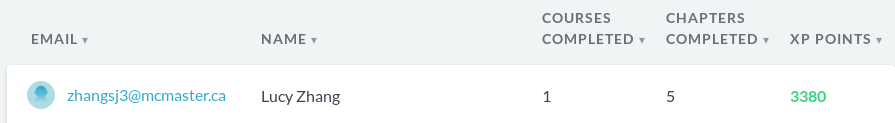
\includegraphics[width=6.5in]{Screenshot_20180911_114301.png}
    \item ~\par
        {
            \renewcommand{\arraystretch}{1.5}
            \noindent \begin{longtable}{p{0.40\textwidth}p{0.60\textwidth}}
                \texttt{echo hello world} & tells the shell to print the content after \texttt{echo} to STDOUT\\
                \texttt{date}             & print the current date to STDOUT\\
                \texttt{hostname}         & print the name of the computer you're on to STDOUT\\
                \texttt{uname -a}         & same as \texttt{uname -mnrsv}, print the name of the operating system (OS), name of the node, the release level of the OS, name of the implementation of the OS, and version of the OS. \\
                \texttt{uptime}           & print the time that the system has been running, number of users logged on and the system load average in the past 1, 5, and 15 minutes\\
                \texttt{whoami}           & print the name of the current user to STDOUT\\
                \texttt{echo \$SHELL}     & print the path to the current shell\\
                \texttt{echo \{con,pre\}\{sent,fer\}\{s,ed\}} & print all the combinations of the items inside the braces to STDOUT\\
                \texttt{clear}            & clears the terminal screen \\
                \texttt{bc -l 41\^ { }73}     & opens a basic calculator that has the standard math library loaded (\texttt{-l}), and performs the calculation\\
                \texttt{echo 5+4 | bc -l}& send 5+4 to basic calculator \\
                \texttt{sleep 5}          & suspend the shell for 5 seconds \\
                \texttt{history}          & show the command history\\
                \texttt{du -sh /home/yourUserID} & estimates the total disk space usage by the files of the home directory and the return value is displayed in human-readable form\\
                \texttt{du -sh /home/yourUserID/\*} & estimate the total disk space usage by each file in the home directory and the return value is displayed in human-readable form\\
            \end{longtable}
        }
    \item ~\par
        {
            \renewcommand{\arraystretch}{1.5}
            \noindent \begin{longtable}{p{0.40\textwidth}p{0.60\textwidth}}
                \texttt{cal}             & prints a small calendar of the current month \\
                \texttt{cal -3}          & prints 3 months spanning the current date\\
                \texttt{cal 9 2018}      & prints the calendar of September 2018 \\
                \texttt{cal 9 1752}      & prints the calendar of September 1752 (start of the Gregorian reformation)\\
                \texttt{cal 28 1 1995}   & Saturday \VerbatimInput{bd.txt}\\
            \end{longtable}
        }
    \item \texttt{chmod} changes the file into an executable for the user.\par
        \VerbatimInput{q4.txt}
    \item \VerbatimInput{q5.txt}
    \item \VerbatimInput{q6.txt}
    \item On info: \texttt{cat /etc/passwd | wc -l}
    \item ~\par
        {
            \renewcommand{\arraystretch}{1.5}
            \noindent\begin{longtable}{lp{0.50\textwidth}}
                \texttt{grep -e 'gene\tb s\{2,\}' Dmelanogaster.gbk} & returns list of genes \\
                \texttt{grep -ce 'gene\tb s\{2,\}' Dmelanogaster.gbk} & returns number of genes \\
                \texttt{37} & \\
                \texttt{grep -ce 'tRNA\tb s\{2,\}' Dmelanogaster.gbk} & returns number of tRNA \\
                \texttt{22} & \\
                \texttt{grep -ce 'rRNA\tb s\{2,\}' Dmelanogaster.gbk} & returns number of rRNA \\
                \texttt{2} & \\
                \end{longtable}
        }
    \item \texttt{grep -ce 'gene\tb s\{2,\}' Bacillus\_genomes/Bacillus\_anthracis\_Ames\_NC\_003997.gbk}\par
        \texttt{5630}\par
        \par
        \texttt{grep -ce 'gene\tb s{2,}' Arabidopsis\_mt.gbk}\par
        \texttt{66}\par
    \item \texttt{grep -ce '\tb d+\tb s.*(t\tb s\{0,1\}a\tb s\{0,1\}t\tb s\{0,1\}t\tb s\{0,1\}a)' Bacillus\_anthracis\_Aes\_NC\_003997.gbk} 
\end{enumerate}

\end{document}
